\chapter{Fase 3: Estudio práctico del test de penetración y análisis del mismo}

\section{Recopilación de información}

En primer lugar, tratamos de recopilar toda la información posible del host de interés. Usando la utilidad "ping" comprobamos que el servidor está operativo y procedemos al escaneo de puertos, para el cual emplearemos \textbf{nmap}.

Metasploitable3, como cualquier servidor real, dispone de varios servicios corriendo en el momento de levantarse. Sin embargo, se encuentra conectada a la red a local a través de una interfaz de Ethernet, y además dispone de un firewall instalado por defecto, lo cual dificulta un poco el análisis.

Suponiendo que no conocemos ninguna IP del servidor metasploitable3, deberíamos comenzar utilizando nmap para un escaneo simple con el objetivo de determinar en qué IP se encuentra escuchando el servidor.

Utilizando la opción \textbf{-sn} (no port scan), indicamos a nmap que queremos hacer un escaneo de la red solo para ver qué hosts se encuentran en ella, así localizaremos nuestro host objetivo. Dado que nuestro propio host (Kali linux) estará también en esta red, añadiremos una opción para excluirlo del escaneo. 

\begin{figure}[hbt]
  \centering
      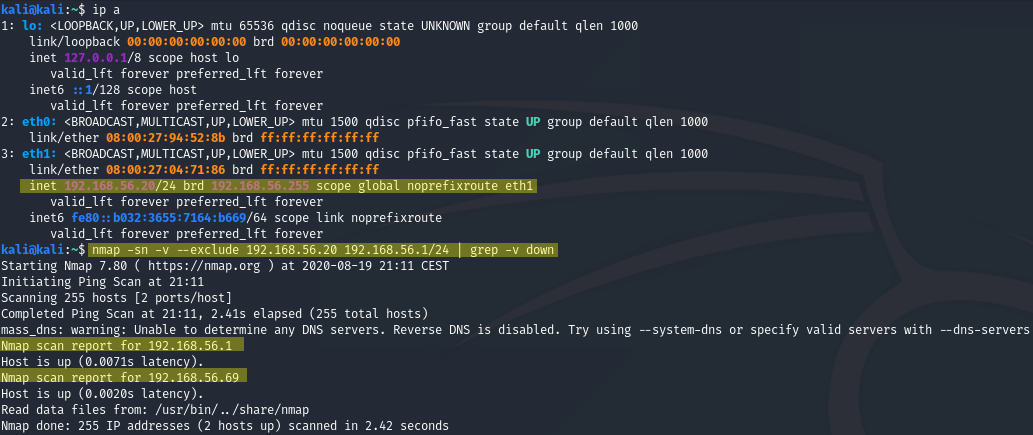
\includegraphics[width=\textwidth]{imagenes/nmap_sn.png}
  \caption{Visualización del escaneo de puertos inicial usando nmap. En él podemos ver que en la red local hay dos nodos además de aquél ejecutando Kali Linux, uno de ellos será el router de la red local (192.168.56.1) y el otro, 192.168.56.69, nuestro objetivo, corriendo metasploit3.}
\end{figure}

A continuación, una vez detectado el nodo que nos interesa, haremos un escaneo más concreto utilizando una opción diferente de nmap, por ejemplo, el flag `-sS`, que realiza un escaneo utilizando TCP sobre un mayor rango de puertos y completando el handshake del protocolo, de forma que puede confirmar qué puertos están abiertos y cuales están cerrados.

